\documentclass[a4paper,12pt]{article}
\usepackage{graphicx}
\usepackage[a4paper, total={6in, 9in}]{geometry}
\usepackage[T1]{fontenc}
\usepackage[utf8]{inputenc}
\usepackage{graphicx}
\usepackage{tikz}
\usepackage{float}
\usepackage{mathtools}
\usepackage{fancyhdr}
\usepackage{caption}
\usepackage{textgreek}
\usepackage{yfonts}
\graphicspath{/home/Desktop/IST/2ano/1semestre/2quarter/SS/relatorio/}
\pagestyle{fancy}
\date{Janeiro-Fevereiro 2022}


\title{Sinais e Sistemas \\ \large {Relatório Laboratorial}}
\author{
\\ João Barreiros C. Rodrigues nº99968
\\Vasco Maria  Aguiar M. R. Esteves nº 100110 }

\begin{document}
	\pagenumbering{gobble}
	\begin{titlepage}
		\maketitle
	\end{titlepage}
	\pagenumbering{arabic}
	\section{Introdução}
	\newpage
	\section{Análise de um sistema (R1-R5)}
		\subsection{Questão R1}
			\paragraph{Da definição algébrica de \textit{linearidade} compreende-se que um sistema linear deve obedecer às condições seguintes:}
				\subparagraph{\textbf{Aditividade:} Ou seja verifica-se que: \textit{sistema(x+y)=sistema(x)+sistema(y)}}
				\subparagraph{\textbf{Homogeneidade: Ou seja verifica-se que: \textit{sistema(}}\textbf{\alpha \textit{y)=} \alpha \textbf{\textit{sistema(y)}}}} \mbox{}\\ \mbox{}\\
			É possível testar a primeira condição executando:
			\begin{figure}[H]
				\centering
					\captionsetup{justification=centering}
					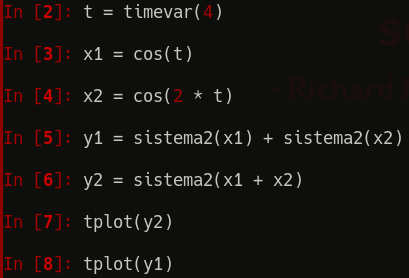
\includegraphics[width=0.5\textwidth]{r1code01.png}
					\caption{Síntese de dois sinais x1 e x2 e síntese de dois sinais y1 e y2 por respectiva soma dos outputs da passagem individual de x1   e x2 pelo sistema 1 e pela passagem do sinal resultante da soma de x1 com x2 pelo sistema1}
			\end{figure}
			Para o qual se obtém o output:
			\begin{figure}[H]
  				\centering
  				\captionsetup{justification=centering}
  				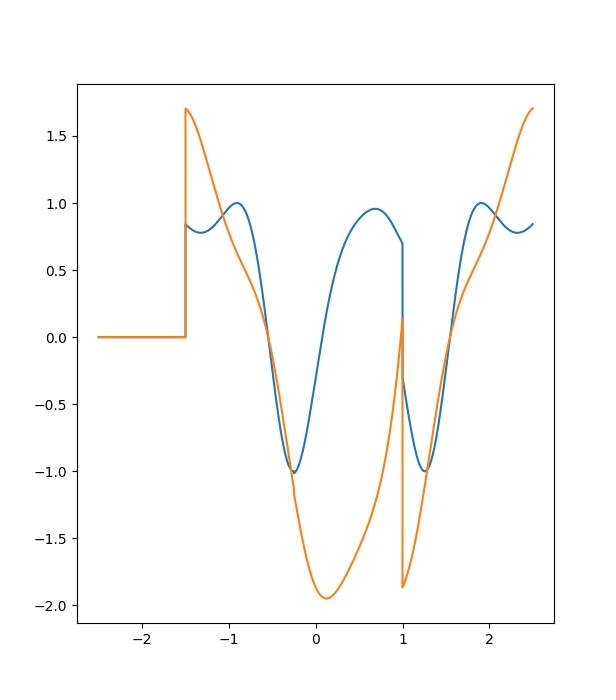
\includegraphics[scale=0.35\textscale]  {r1graph01.png}
				\caption{A azul e a verde, respectivamente as representações gráficas de y1 e y2, de notar que y1 \neq y2}
			\end{figure}
			Verificando assim que o sistema não é aditivo, precipitando para a conclusão da  \textbf{não-linearidade do sistema.}\\
			Embora a linearidade seja uma conjunção de duas propriedades, realiza-se também o teste da condição de homogeneidade para efeitos de estudo:
 			\begin{figure}[H]
  				\centering
  				\captionsetup{justification=centering}
  				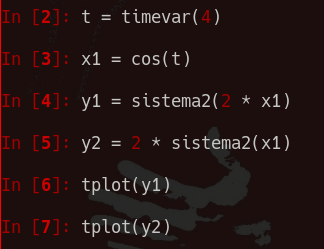
\includegraphics[width=0.3\textwidth]{r1code02.png}
				\caption{Síntese de um sinal x1 e síntese de dois sinais y1 e y2 por respectiva passagem do produto de x1 com uma contante \textbeta (tal que \textbeta =2) pelo sistema 2 e pelo produto do resultado da passagem de x1 pelo sistema 2 com \textbeta}
  			\end{figure}
			Para o qual se obtém os outputs:
			\begin{figure}[H]
    				\centering
    				\captionsetup{justification=centering}
    				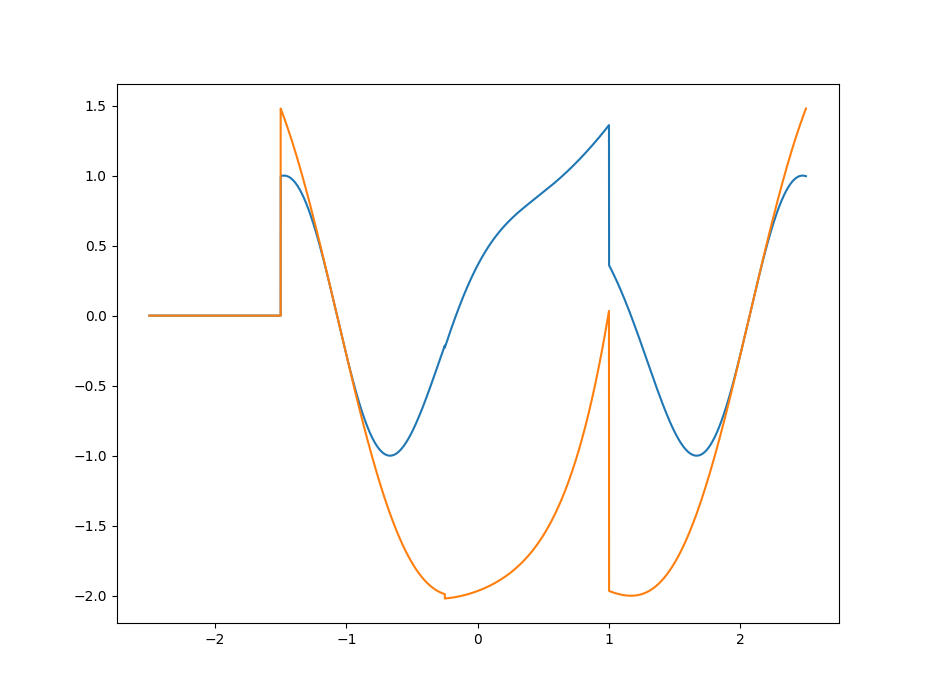
\includegraphics[scale=0.4\textscale]  {r1graph02.png}
				\caption{A azul e a laranja, respectivamente as representações gráficas de y1   e y2, de notar que y1 \neq y2}
  			\end{figure}
			Provando adicionalmente que o sistema \textbf{não é homogéneo}
			\newpage
		\subsection{Questão R2}
			\paragraph{Definem-se sistemas invariantes no tempo aqueles que não dependem directamente da variável tempo, ou seja na expressão matemática do sistema não está comtemplada a variável tempo. O sistema invariante no tempo pode contudo depender indirectamente do tempo, ou seja a função de \textit{input} dada pode depender explicitamente do tempo.}
			\mbox{}\\
			\mbox{}\\
			Desta forma, o mais simples teste que se pode realizar de forma a concluir a variância ou invariância no tempo de um sistema é através do deslocamento do sinal de entrada.
			O sistema será invariante no tempo se a seguinte proposição for verdadeira:
			\mbox{}\\
			\mbox{} \\
			\mbox{		} \textit{Para x$_0$(t) e x$_1$(t)=x$_0$(t+\textbeta) ou seja x$_1$(t)= \mathbb{T}$_\textbeta$ x$_0$(t)
			\\ 
			\mbox{          } \mathbb{T}$_\textbeta$ sistema(x$_0$)=sistema(x$_1$)}
			\mbox{}\\
			\mbox{          } Considerando \mathbb{T}$_\textbeta$ o operador deslocamento para o vector (0,-\textbeta)
\mbox{}\\\mbox{}\\
			Tomando as noções anteriores computa-se no ambiente \textit{ipython}:
			\begin{figure}[H]
    				\centering
    				\captionsetup{justification=centering}
    				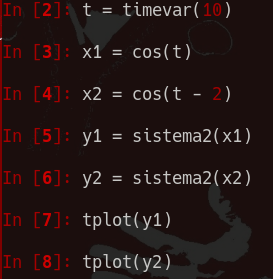
\includegraphics[width=0.3\textwidth]{r2code01.png}
				\caption{Síntese de um sinal x1 e  x2, tal que x2=\mathbb{T} $_-$$_2$ e síntese de dois sinais y1 e y2 por respectiva passagem de x1 e x2 pelo sistema2}
    			\end{figure}
			Para o qual se obtém os outputs:
 			\begin{figure}[H]
      				\centering
      				\captionsetup{justification=centering}
      				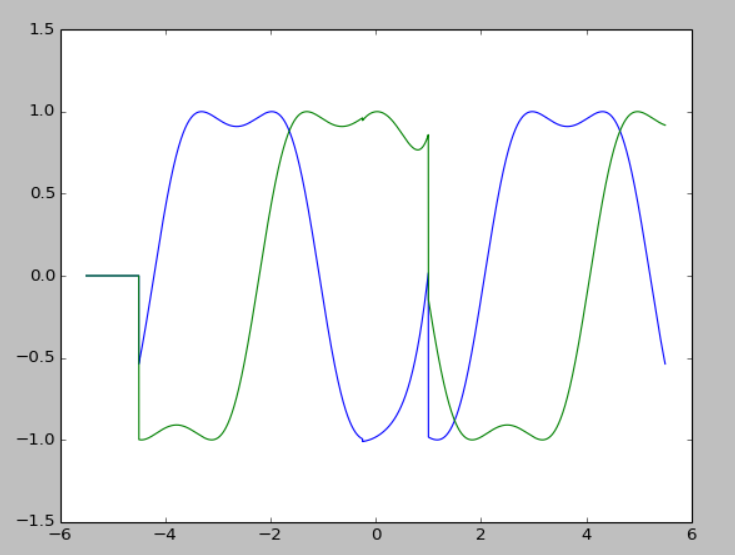
\includegraphics[scale=0.3\textscale]{r2graph.png}
				\caption{A azul e a verde, respectivamente, os sinais y1 e y2. De notar a distinção entre a forma de onda de y1 e y2, indiciando que \mathbb{T} $_-$$_2$ y1\neq y2}
      			\end{figure}
			Concluindo-se que o sistema 2 \textbf{não é invariante no tempo}
	\newpage	
	\subsection{Questão R3}
		\paragraph{Sucintamente, um sistema descreve-se como sem memória se o seu output para um instante t$_1$ for dependente apenas do input dado nesse mesmo instante.}
		\mbox{}\\
		\mbox{}\\
		Desta forma é possível aferir que um sistema sem memória tem todas as suas referências canônicas à variável tempo na forma:
		\\ 
		\begin{center}
			\textalpha $t^{\gamma}$ +\textbeta , com \textalpha = 1, \textgamma=1 e \textbeta=0.
		\end{center}
		\\
		Um teste simples que pode ser utilizado para verificar esta propriedade consiste na síntese de dois sinais x$_0$ e x$_1$ distintos que se intersetam em determinado instante t$_i$. Para um sistema de equação y$_1$ o sistema será sem memória se y$_1$(x$_0$) e y$_1$(x$_1$) se intersetarem em t$_i$.
		\mbox{}\\
		\mbox{}\\
		Executando o referido teste:
		\begin{figure}[H]
      			\centering
      			\captionsetup{justification=centering}
      			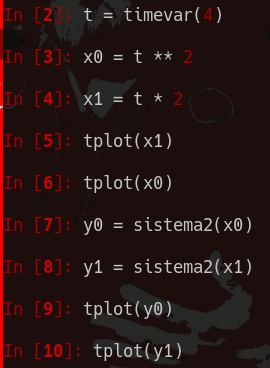
\includegraphics[width=0.2\textwidth]{r3code01.png}
			\caption{Realização em ambiente \textit{ipython} do teste acima descrito}
      		\end{figure}
		Do qual se obtém o primeiro \textit{output}, de controlo:
		\begin{figure}[H]
        		\centering
        		\captionsetup{justification=centering}
        		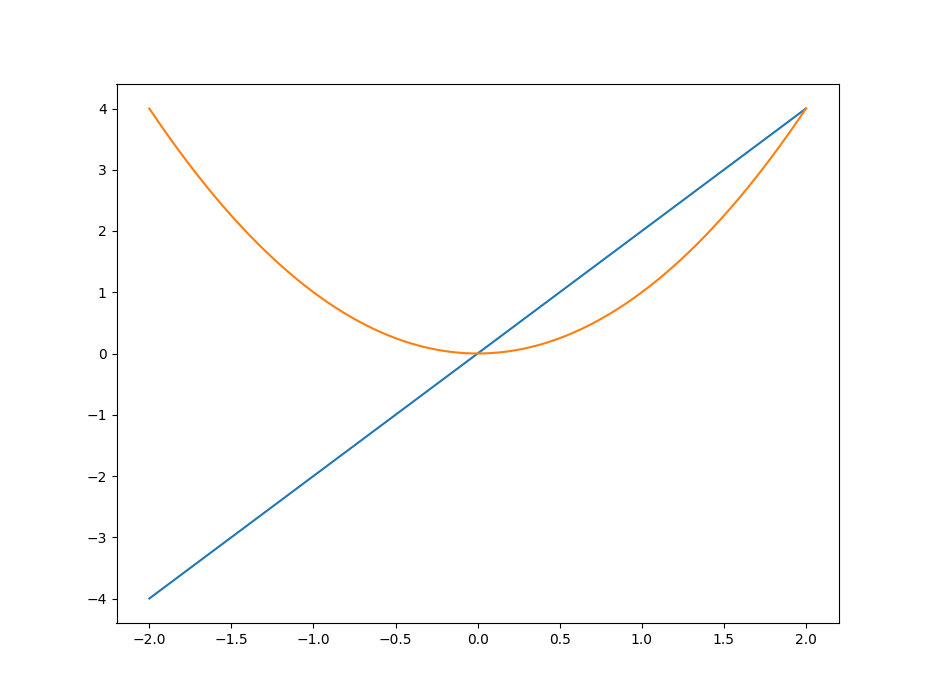
\includegraphics[scale=0.35\textscale]{r3graph01.png}
			\caption{Representação gráfica de x1 (a azul) e x0 (a laranja). De notar a intersecção dos gráficos para t=0 e t=2}
        	\end{figure}
		E o segundo, conclusivo:
		\begin{figure}[H]
       	 		\centering
        		\captionsetup{justification=centering}
        		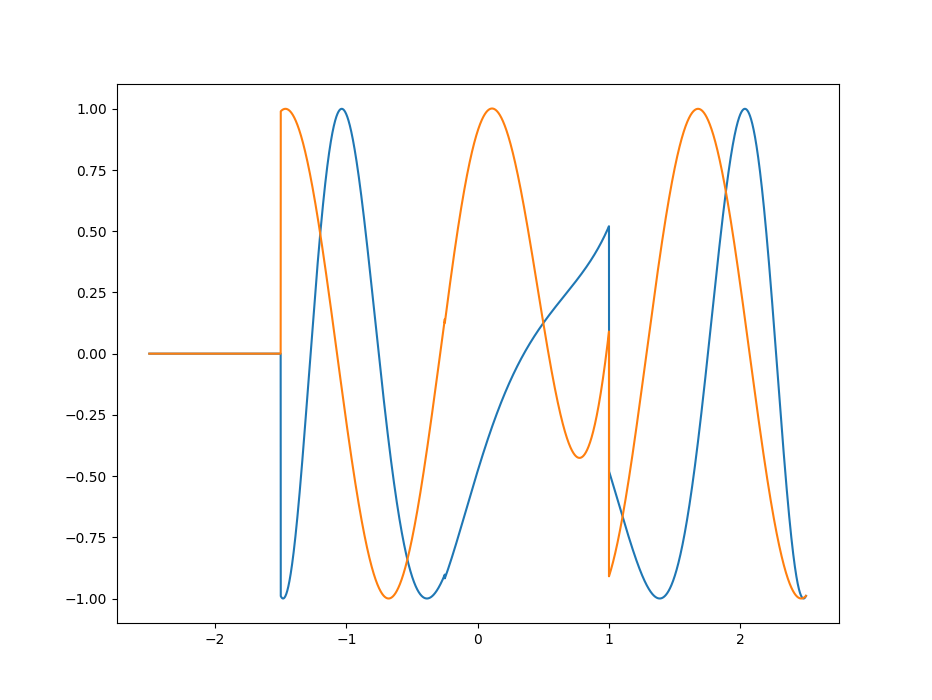
\includegraphics[scale=0.35\textscale]{r3graph02.png}
			\caption{Representação gráfica de y0 (a azul) e y1 (a laranja). Verifique-se a não intersecção do gráficos em t=0 e t=2}
		\end{figure}
		Prova-se que o sistema 2 \textbf{é com memória}
	\subsection{Questão R4}
		\paragraph{Assim como na caracterização da memória do sistema, também a definição de causalidade assenta nas particularidades do sistema relativas à variável tempo. Desta forma um sistema descreve-se como causal quando o  seu output para qualquer instante t$_1$ for dependente apenas de inputs presentes ou passados ou seja t$_1$ \ge t _{input}}\mbox{  }\\ \mbox{}\\
		Desta forma é possível aferir que um sistema causal tem todas as suas referências canônicas à variável tempo na forma:\\
		\begin{center} 
			\begin{math}
				\textalpha t^{\gamma}$ +\textbeta , com \textalpha \in ]0,1[, \gamma \in ]0,  1] \mbox{  }e \mbox{  }\beta  \in ]- \infty , 0]. 
			\end{math}
		\end{center}
		\\

	\subsection{Questão R5}
\end{document}
